\section{Monte Carlo Arithmetic: Polynomial evaluation}

Polynomial evaluation is a common source of computational error. Polynomials are
frequently used for function interpolation in libraries or user codes.
Different evaluations of the same polynomial do not have the same
behavior in terms of performance or numerical accuracy.

This tutorial uses the Tchebychev polynomial from ~\cite[pp.52-54]{parker1997monte}:

$$T(x)=\sum_{i=0}^{10}{a_i \times x^{2i}}$$
With:
$a_i \in [
    1,
    \matminus 200,
    6600,
    \matminus 84480,
    549120,
    \matminus 2050048,
    4659200,
    \matminus 6553600,
    5570560,
    \matminus 2621440,
    524288
  ]$

Due to catastrophic cancellations, the polynomial is difficult to evaluate near
$1$ as discussed in~\cite[pp.52-54]{parker1997monte}.

\subsection{Evaluation of the naive expanded form}

\subsubsection{First steps with Verificarlo}

In this first approach, we will evaluate the polynomial in its expanded naive
form and in single precision. This part of the tutorial is located in the
\texttt{tchebychev/} folder.

\begin{question}
  \begin{enumerate}[(a)]
    \item Open the {\tt tchebychev.c} file and observe the function {\tt REAL expanded(REAL x)}.

    \item Compile {\tt tchebychev.c} with {\tt verificarlo} using the following command:
          \begin{verbatim}
verificarlo -D FLOAT tchebychev.c -o tchebychev
\end{verbatim}
    \item Run the program.
  \end{enumerate}
\end{question}

You should get an error as the \texttt{VFC\_BACKENDS} environment variable is empty.
The simplest backend is the one emulating IEEE-754 arithmetic(\texttt{libinterflop\_ieee.so}).
It has a \texttt{-{}-debug} option that trace each instrumented floating-point operations.

\begin{question}
  Run the program using the IEEE backend,
  \begin{verbatim}
VFC_BACKENDS="libinterflop_ieee.so --debug" ./tchebychev 0.99 EXPANDED
\end{verbatim}
\end{question}

To estimate the numerical error, we will now use the Monte Carlo Arithmetic
backend (\texttt{libinterflop\_mca.so}) in single precision by simulating
round-off errors that could occurs at 24 bits of precision.

\begin{question}
  \begin{enumerate}[(a)]

    \item Run the program using the Monte Carlo Arithmetic backend with 24 bits
          precision for single precision variables,
          \begin{verbatim}
VFC_BACKENDS="libinterflop_mca.so --precision-binary32=24" ./tchebychev 0.99 EXPANDED
\end{verbatim}
    \item Execute the program multiple times. What can you observe?
  \end{enumerate}
\end{question}

The Monte Carlo Arithmetic backend define precision (i.e. noise level) for
single and double precision variable by respectively using the
\texttt{-{}-precision-binary32=<value>} and
\texttt{-{}-precision-binary64=<value>}.

The Monte Carlo arithmetic backend supports different modes,
\begin{itemize}

  \item \texttt{-{}-mode=rr} is the \emph{random round} mode that adds noise on the
        result of an operation only when the operation is not exactly representable
        at the chosen precision. This mode is useful to simulate the effect of
        round-off errors.

  \item \texttt{-{}-mode=pb} is the \emph{precision bound} mode that adds noise on
        the operands before performing the operation. It is useful to simulate the
        effect of cancellations errors.

  \item \texttt{-{}-mode=mca} is the default mode that combines \texttt{rr} and
        \texttt{pb} modes.

\end{itemize}

%\begin{question}
%  \begin{enumerate}[(a)]
%    \item Now recompile with verificarlo the program in double precision using the command:\newline
%          {\tt verificarlo -D DOUBLE tchebychev.c -o tchebychev} \\
%    \item Execute the program with arguments \texttt{0.99 EXPANDED} with the Monte Carlo arithmetic backend. Try different precisions such as 53, 24, 10. Try also to use different modes (rr, pb, mca). What do you observe?
%  \end{enumerate}
%\end{question}

\subsubsection{Numerical quality analysis}

In this section, we analyze the numerical quality of the computed results.  The
\texttt{run.sh} script available in the exercice directory automates the
verificarlo runs.  Visualization is done using the \texttt{plot.py} script.

Since we are working with a headless docker image, the \texttt{plot.py} output
will be a \texttt{.pdf} file that you can open in the host machine.

\begin{question}
  \begin{enumerate}[(a)]
    \item Open {\tt run.sh} and understand how it works.
    \item Modify {\tt run.sh} to evaluate the polynomial in the interval $[0.5,1]$ by $0.001$ step (you can leave the number of execution unchanged).
    \item Open {\tt plot.py} and understand how it works, and what are the plotted data.
  \end{enumerate}
\end{question}

Table~\ref{fig:exp_24_53} is generated with the \texttt{plot.py} script.

The lowest part of each plot shows the $T(x)$ samples and their average in dotted line. The 20 Monte Carlo samples $T(x)$ are plotted for each $x$ value (sometimes overlapping on the graphic).
The central part is the empirical standard deviation $\hat\sigma$ for each value of $x$.
The upper part of the figure represents the number $s$ of significant digits of each output defined as $s=-\log_{10}\left|\dfrac{\hat\sigma}{\hat\mu}\right|$ with $\hat\sigma$ the sample empirical standard deviation and $\hat\mu$ their average.

\begin{question}
  \begin{enumerate}[(a)]
    \item To execute the {\tt EXPANDED} version with {\tt float (binary32)} types and a virtual precision of 24 bits, execute the command: {\tt ./run.sh EXPANDED FLOAT 24 mca} \newline
          This command's output is given in table~\ref{fig:exp_24_53} (Left).
    \item Now execute the benchmark with {\tt double (binary64)} types and a virtual precision of 53. You can use
          the command: {\tt ./run.sh EXPANDED DOUBLE 53 mca} \newline
          This command's output is given in table~\ref{fig:exp_24_53} (Right).
    \item Compare the number $s$ of significant digits in both cases. What is the problem and is double precision a solution?
  \end{enumerate}
\end{question}

\begin{table}
  \begin{tabular}{cc}
    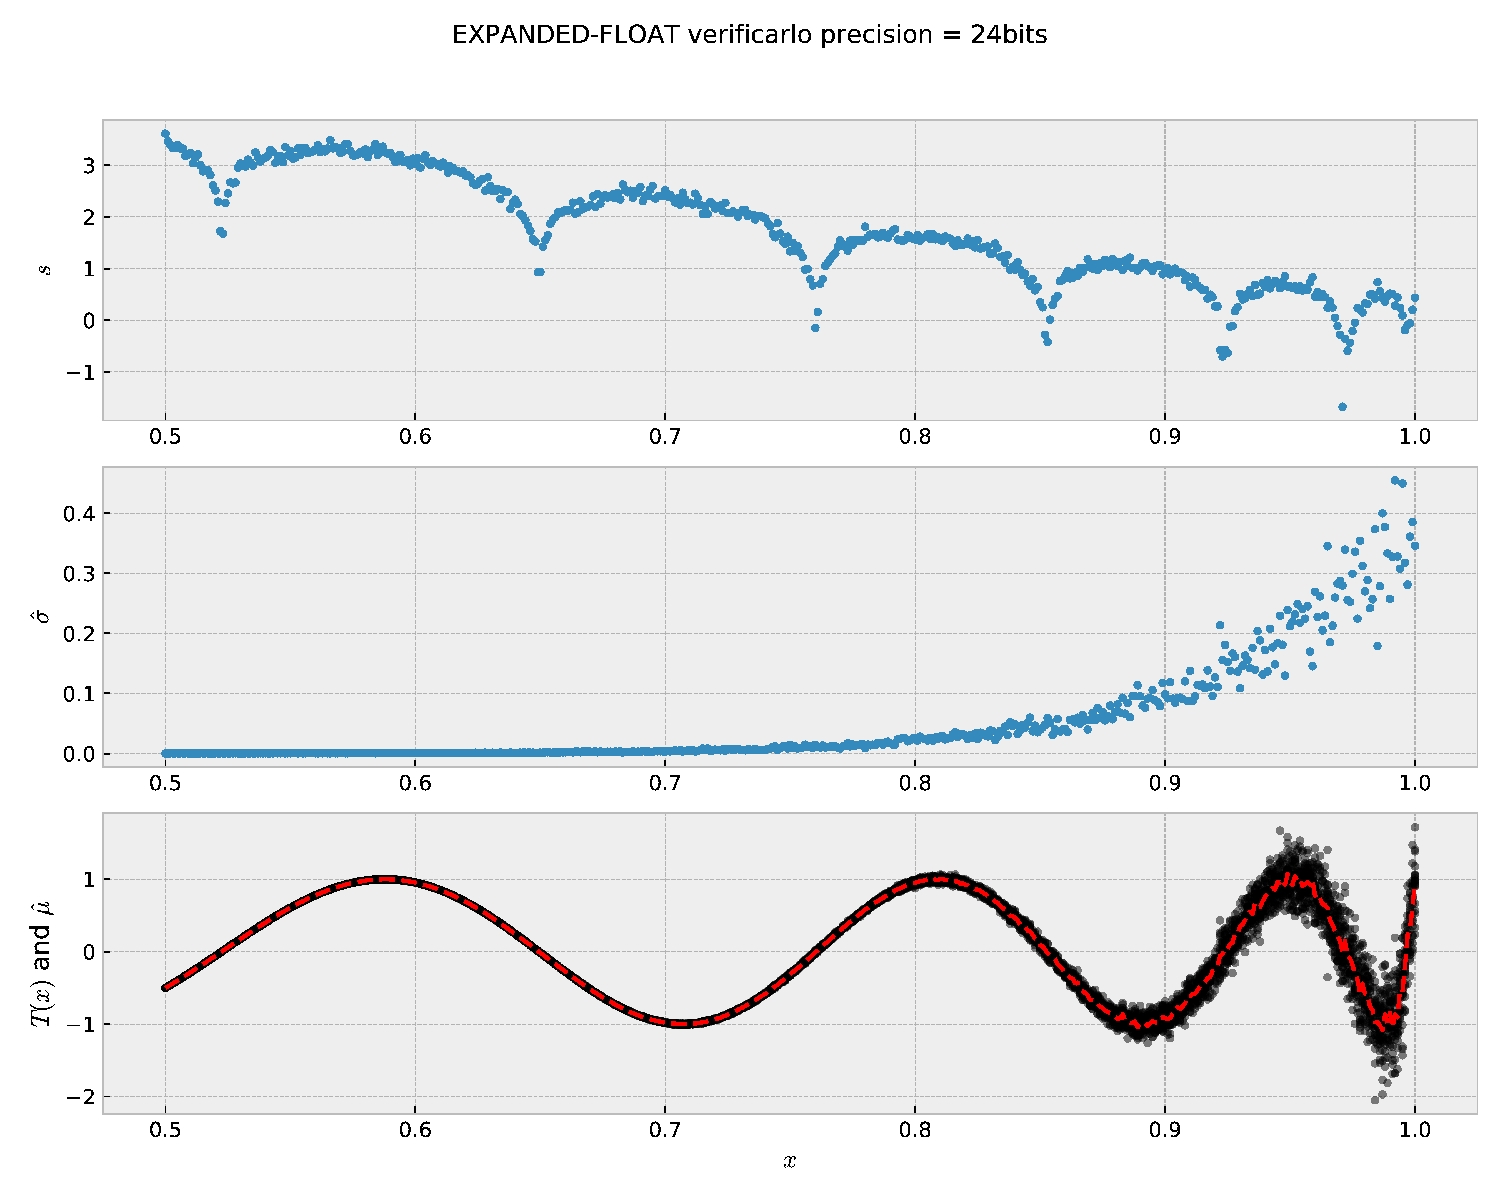
\includegraphics[width=.47\textwidth]{EXPANDED-FLOAT-24.pdf} &
    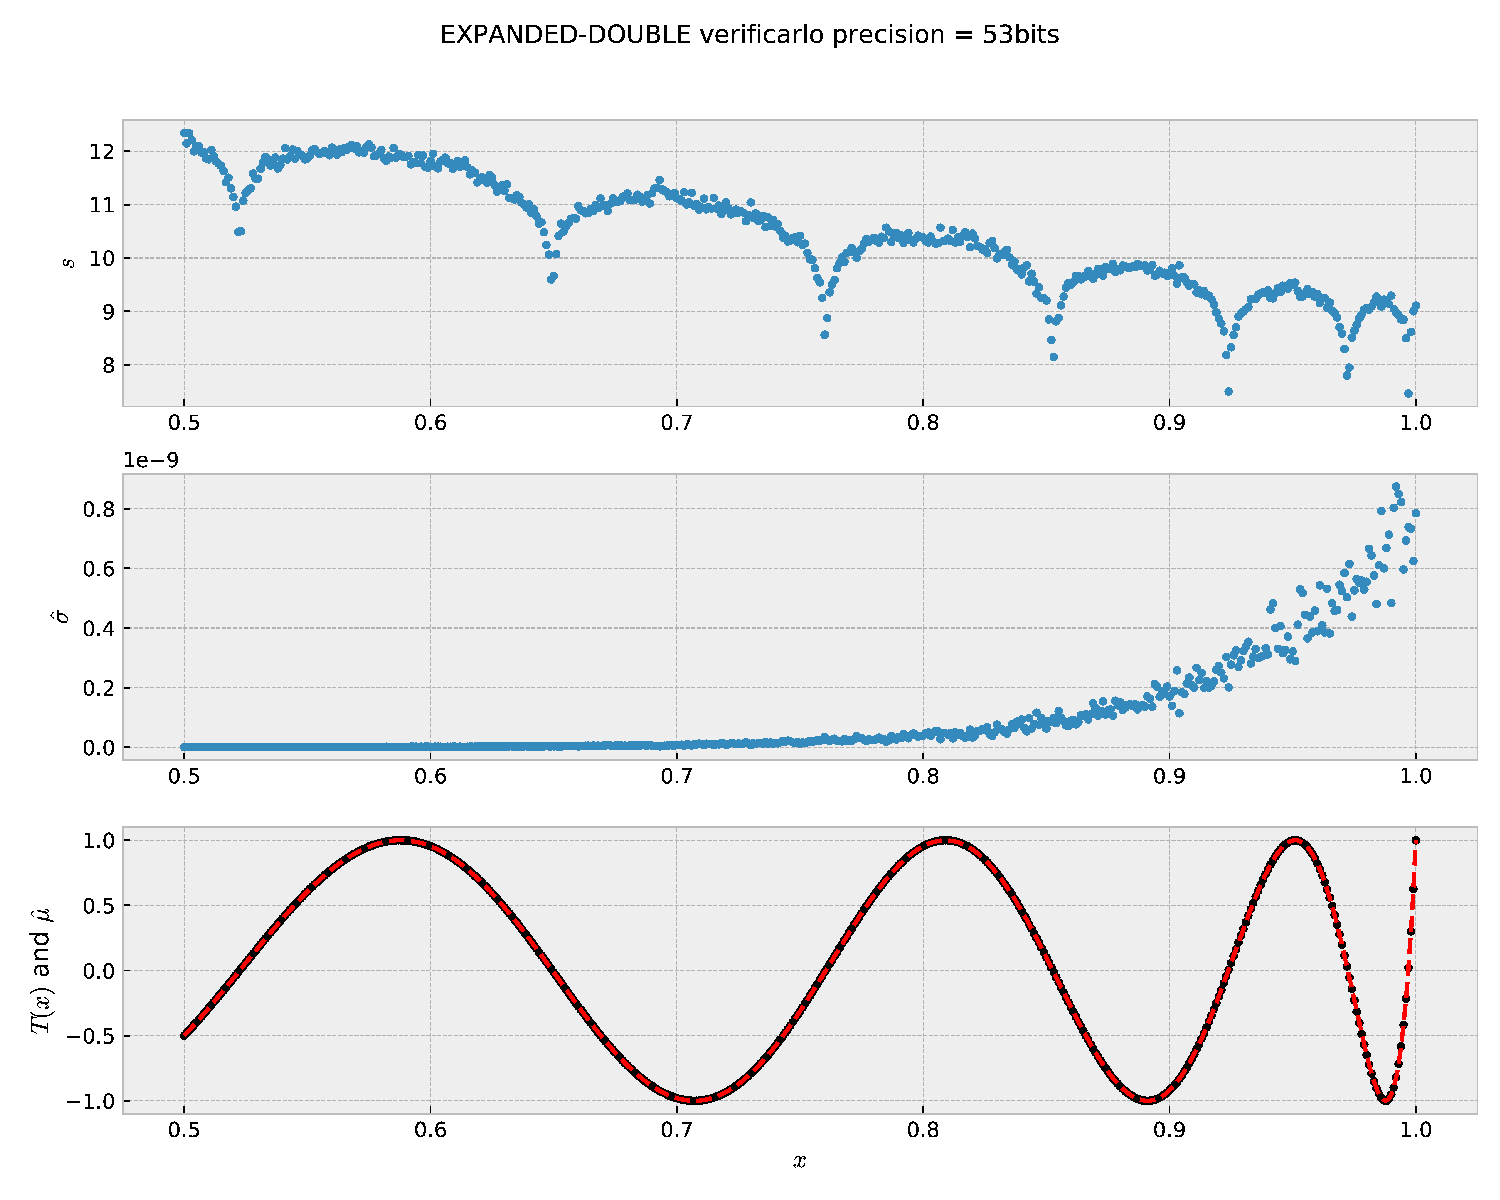
\includegraphics[width=.47\textwidth]{EXPANDED-DOUBLE-53.pdf}  \\
    %Expanded form, 24 bits & Expanded form, 53 bits \\
  \end{tabular}
  \caption{Evaluation of T(x) in Expanded form, compiled in single/double precision, with a virtual precision of 24/53 bits}
  \label{fig:exp_24_53}
\end{table}

The polynomial evaluation done with 24 bits is subject to severe {\it cancellations} when the input value is close to $1$.
This drasticaly reduces the accuracy of the result.
Using evaluation in double precision on the contrary seems satisfactory. But
this solution forces the developer to use a larger and more expensive data type
and it does not solve the problem, it only delays it.

\FloatBarrier

